% !TeX program = pdflatex
\documentclass[border=6pt]{standalone}
\usepackage{tikz}
\usetikzlibrary{arrows.meta, positioning}

\definecolor{MediumRed}{rgb}{0.925, 0.345, 0.345}
\definecolor{MediumGreen}{rgb}{0.37, 0.7, 0.66}
\definecolor{MediumBlue}{rgb}{0.015, 0.315, 0.45}
\definecolor{DarkBlue}{rgb}{0.05, 0.15, 0.35}

\begin{document}
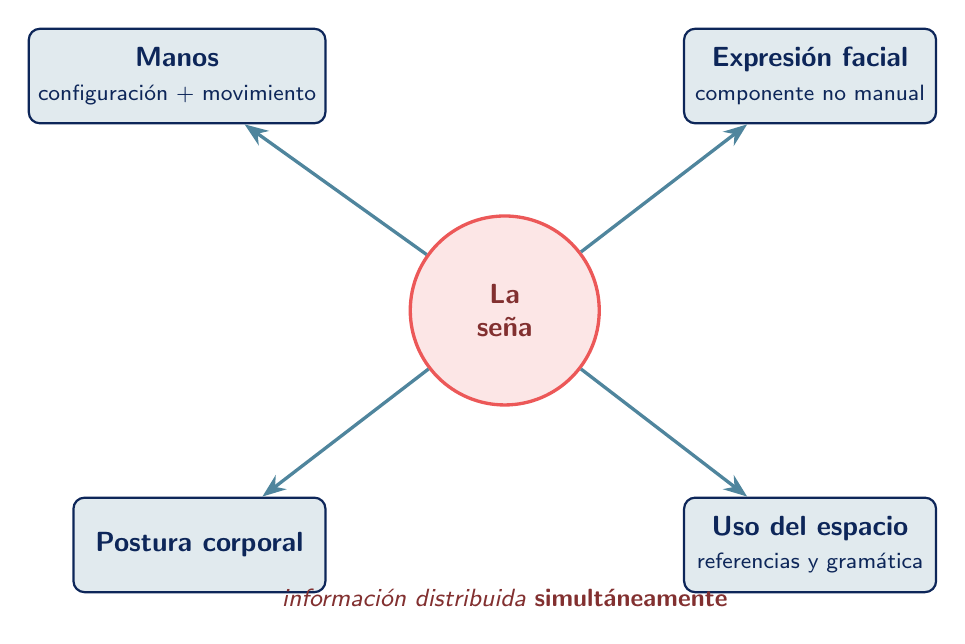
\begin{tikzpicture}[
    font=\sffamily,
    channel/.style={draw=DarkBlue, thick, rounded corners=4pt,
        fill=MediumBlue!12, align=center, text=DarkBlue,
        minimum width=3.2cm, minimum height=1.2cm},
    link/.style={-{Stealth[length=3mm]}, line width=1.2pt, MediumBlue!70},
]

% nucleo
\node[circle, draw=MediumRed, very thick, fill=MediumRed!15,
      text=MediumRed!55!black, font=\sffamily\bfseries, align=center,
      minimum size=2.4cm] (core) {La\\seña};

% cuatro canales simultaneos
\node[channel, above left=1.5cm and 1.4cm of core]  (hands)
    {\textbf{Manos}\\\footnotesize configuración + movimiento};
\node[channel, above right=1.5cm and 1.4cm of core] (face)
    {\textbf{Expresión facial}\\\footnotesize componente no manual};
\node[channel, below left=1.5cm and 1.4cm of core]  (body)
    {\textbf{Postura corporal}};
\node[channel, below right=1.5cm and 1.4cm of core] (space)
    {\textbf{Uso del espacio}\\\footnotesize referencias y gramática};

\draw[link] (core) -- (hands);
\draw[link] (core) -- (face);
\draw[link] (core) -- (body);
\draw[link] (core) -- (space);

% etiqueta de simultaneidad
\node[font=\sffamily\small\itshape, text=MediumRed!55!black, below=2.2cm of core]
    {información distribuida \textbf{simultáneamente}};

\end{tikzpicture}
\end{document}
